\documentclass{beamer}
\usepackage{tikz}
\usetikzlibrary{shapes,arrows}
\usepackage{fancyvrb}
\usepackage{graphics}
\usetheme{default}
\title{Write-and-f-array: implementation and an application}
\author{Robert Obryk}
\date{September 2013}
\fvset{commandchars=\\\{\}}
\begin{document}
\frame{\titlepage}
\begin{frame}[fragile]{Snapshot}
\begin{Verbatim}
var T: array[0..N-1] of X
read():
  return T
update(i, x):
  T[i] <- x
\end{Verbatim}
\end{frame}
\begin{frame}[fragile]{F-array}
\begin{Verbatim}
var T: array[0..N-1] of X
read():
  return \textcolor{red}{T[0] + T[1] + ... + T[N-1]}
update(i, x):
  T[i] <- x
\end{Verbatim}
\end{frame}
\begin{frame}[fragile]{Write-and-snapshot}
\begin{Verbatim}
var T: array[0..N-1] of X
read():
  return T
update\textcolor{green}{-and-read}(i, x):
  T[i] <- x
  \textcolor{green}{return T}
\end{Verbatim}
\end{frame}
\begin{frame}[fragile]{Write-and-f-array}
\begin{Verbatim}
var T: array[0..N-1] of X
read():
  return \textcolor{red}{T[0] + T[1] + ... + T[N-1]}
update\textcolor{green}{-and-read}(i, x):
  T[i] <- x
  \textcolor{green}{return} \textcolor{red}{T[0] + T[1] + ... + T[N-1]}
\end{Verbatim}
\end{frame}
\begin{frame}{Interlude: Implementation of The F-array}
\begin{tikzpicture}
\node(root) at (0, 0) {\textcolor<6>{purple}{T[0] + ... + T[N-1]}};
\node(left) at (-3, -2) {T[0] + ... + T[N/2-1]};
\node(right) at (3, -2) {\textcolor<5-6>{purple}{\textcolor<3-4>{red}{T[N/2] + ... + T[N-1]}}};
\draw (root) to (left);\draw(root) to (right);
\node(ll) at (-4, -4) {...};
\node(lr) at (-2, -4) {...};
\draw(left) to (ll);\draw(left) to (lr);
\node(rr) at (4, -4) {\textcolor<4-6>{blue}{...}};
\node(rl) at (2, -4) {\textcolor<2-6>{red}{...}};
\draw(right) to (rl);\draw(right) to (rr);
\draw<7>(-5,-5) rectangle (-1,-1);
\draw<7>(5,-5) rectangle (1,-1);
\end{tikzpicture}
\end{frame}

\begin{frame}[fragile]{Interlude: Implementation of The F-array}
\begin{Verbatim}
var C: array[0..1] of f-array
var V: X

percolate():
  LL(V)
  V' := C[0].read() + C[1].read()
  return SC(V, V')

update(i, x):
  C[...].update(..., x)
  if not percolate():
    percolate() // ignore failure

read():
  return V
\end{Verbatim}
\end{frame}

\begin{frame}{Update timing}
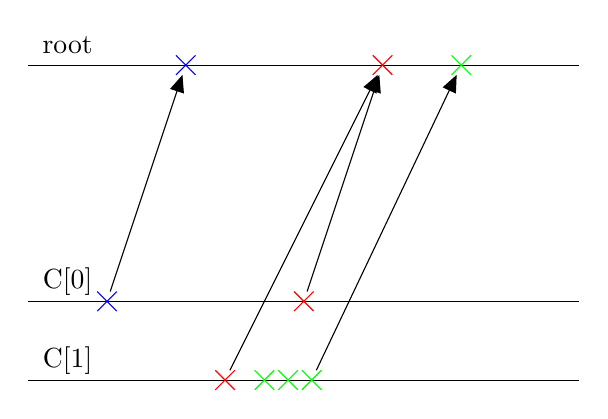
\begin{tikzpicture}
\node(rootbeg) at (0.5,0.25) {root};
\draw(0,0) to (7,0);
\node(c0beg) at (0.5,-2.75) {C[0]};
\draw(0,-3) to (7,-3);
\node(c1beg) at (0.5,-3.75) {C[1]};
\draw(0,-4) to (7,-4);

\node<1->[cross out,draw=blue](c0-0) at (1, -3) {};
\node<1->[cross out,draw=blue](root-0) at (2, 0) {};
\draw<1->[arrows={-triangle 45}] (c0-0) to (root-0);


\node<3->[cross out,draw=red](c0-1) at (3.5, -3) {};
\node<2->[cross out,draw=red](c1-1) at (2.5, -4) {};
\node<3->[cross out,draw=red](root-1) at (4.5, 0) {};
\draw<3->[arrows={-triangle 45}] (c1-1) to (root-1);
\draw<3->[arrows={-triangle 45}] (c0-1) to (root-1);

\node<2->[cross out,draw=green](c1-2-a) at (3, -4) {};
\node<2->[cross out,draw=green](c1-2-b) at (3.3, -4) {};
\node<4->[cross out,draw=green](c1-2) at (3.6, -4) {};
\node<4->[cross out,draw=green](root-2) at (5.5, 0) {};
\draw<4->[arrows={-triangle 45}] (c1-2) to (root-2);
\end{tikzpicture}
\end{frame}

\begin{frame}[fragile]{The History Object}
Represents an infinite append-only log. Entries are indexed by consecutive \emph{version numbers}
\begin{itemize}
\item \verb+get_current(): (version, value)+ -- returns the most recent entry
\item \verb+publish(version, value): bool+ -- publishes a given entry iff the current one has the previous version number
\item \verb+get(version): maybe value+ -- returns a value stored with a given version number, if sufficiently recent
\end{itemize}
\end{frame}

\begin{frame}[fragile]{Write-and-f-array: First attempt}
\begin{Verbatim}
var C: array[0..1] of f-array
var V: \textcolor{red}{HistoryObject(X)}

percolate():
  \textcolor{red}{version, value := V.get_current()}
  value' := C[0].read() + C[1].read()
  return \textcolor{red}{V.publish(version + 1, value')}

update(i, x):
  \textcolor{red}{value := }C[...].update(..., x)
  if not percolate():
    percolate() // ignore failure
  \textcolor{red}{Find the first history element that includes this update}
  \textcolor{red}{Combine it with value}

read():
  return \textcolor{red}{V.get_current().value}
\end{Verbatim}
\end{frame}

\begin{frame}[fragile]{Write-and-f-array: Handle stragglers}
Idea: Let's \emph{help} everyone complete their operation
\begin{itemize}
\item In turns: one array element per successful \verb+publish+.
\item We need his data: extend the interface to cover this.
\item We are reduced to one concurrent \verb+update(i, x)+ for any
given \verb+i+.
\end{itemize}
\end{frame}

\begin{frame}{Time and Space Complexities}
$N$ is the array's size.

\begin{tabular}{|l||l|l|}
\hline
Memory & $O(N \lg N)$ & $O(N \lg^2 N)$\\
Time of \verb+update+ & $O(\lg^3 N)$ & $O(\lg^2 N)$\\
Time of \verb+read+ & $O(1)$ & $O(1)$ \\
\hline
\end{tabular}
\end{frame}

\begin{frame}[fragile]{Fetch-and-add}
\begin{Verbatim}
var V: int

fetch-and-add(delta):
  V = V + delta
  return V - delta
\end{Verbatim}

Our implementation for $P$ threads:
\begin{itemize}
\item $O(P \log P)$ memory (subquadratic)
\item $O(\log^3 P)$ time (polylogarithmic)
\end{itemize}
\end{frame}

\begin{frame}{Experimental results}
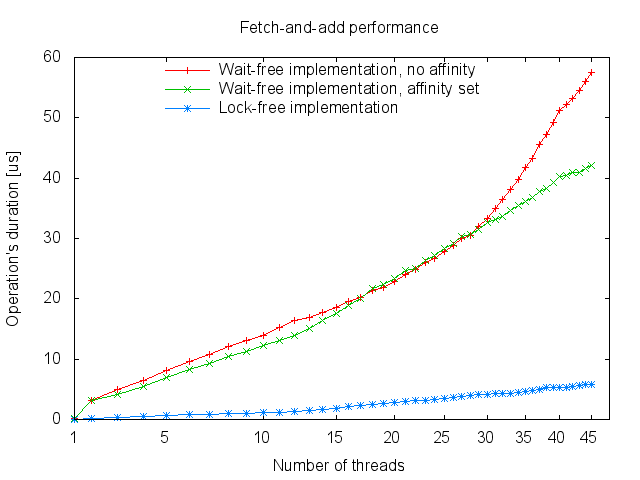
\includegraphics[scale=0.6]{meas.png}
\end{frame}

\begin{frame}{}
Thank you for your attention. Questions?
\end{frame}

\end{document}
